\documentclass[../writeup.tex]{subfiles}

\begin{document}  

\section{Details}
 
\subsection{Structured Light Stereo}

Some relevant reiews are \cite{salviPatternCodificationStrategies2004},\cite{salviStateArtStructured2010} and \href{http://www.sci.utah.edu/~gerig/CS6320-S2013/Materials/CS6320-CV-S2012-StructuredLight-II.pdf}{slides}. A \textit{structured light stereometric system} is similar to a passive stereo system where one of the camera is replaced by a projector. A light source projects light a vertical plane of light that creates a narrow stripe on the scene. The intersection of an illumination plane of known spatial position (corresponds to a projector column) and a line of sight (corresponds to a camera pixel) determines a point. For dense reconstruction of the scene, many images must be taken. To speed up the scanning process, spatially modulated light projector has been suggested, in which multiple illumination planes or rays can be projected simultaneously as part of a single illumination pattern. Spatial-temporal modulation of illumination, i.e. sequentially projecting several patterns, can be used for reliable identification of light planes. To enable acquisition of dynamic scenes, the number of projected patterns used should be as small as possible. Intuitively, the projected pattern impose illusion of texture on the object, increasing the number of correspondences, which enables reconstruction. Structured light stereo is equivalent to (1) solving the correspondence problem and then (2) computing stereo using triangulation.


\subsubsection{The Correspondence Problem}

The correspondence problem can be stated simply
\begin{center}
    \textit{
        For each point in the left image, find the corresponding point in the right image
    }
\end{center}
We first note that search space for the corresponding point can be restricted to pixels lying on the epipolar line. Epipolar plane is plane formed from points $p,o_1,o_2$ and epipolar line is intersection of epipolar plane with the image plane.
\begin{figure}[h!]
    \begin{center}
        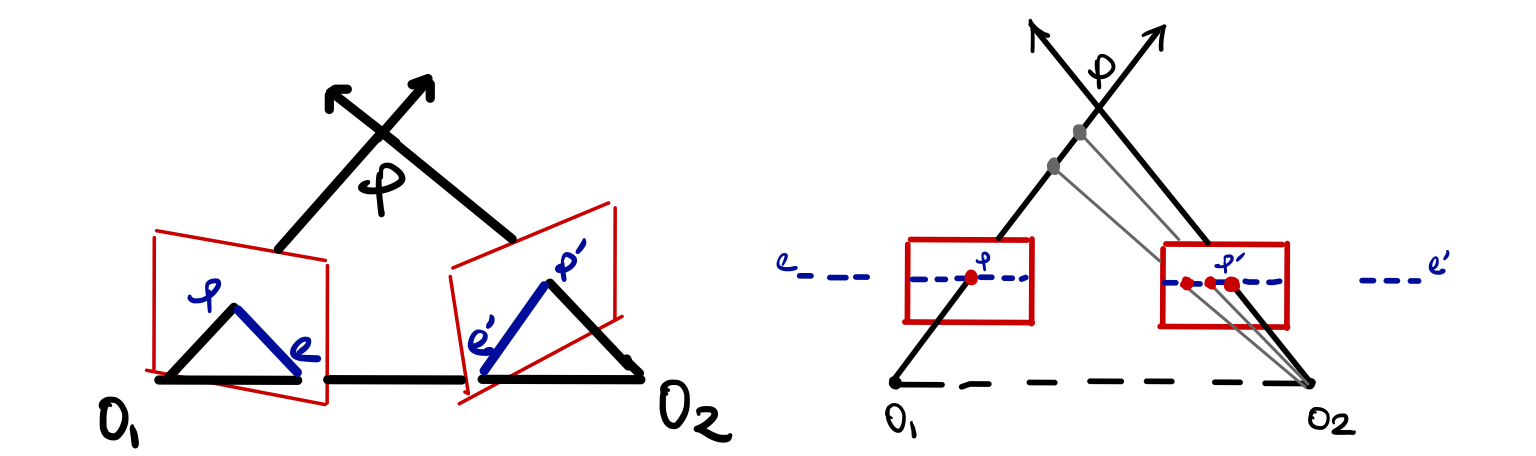
\includegraphics[width=4in]{epipolar_constraint_correspondence}
        \caption{non parallel (left) and parallel (right) camera setup. $pe$ and $p'e'$ are the epipolar lines}
    \end{center}
\end{figure}
For structured light stereo systems, the art of designing robust, fast, reliable coding schemes serves to solve the correspondence problem.


\subsubsection{Triangulation}

Given correspondence between projector and camera images, triangulation refers to the process of computing the distance of object relative to camera. Since a 3D point can be obtained by intersecting a ray (pixel of camera image) with a projector plane (a single code), it is necessary to encode a single axis in projected image to ensure unique reconstruction. 
\begin{figure}[h!]
    \begin{center}
        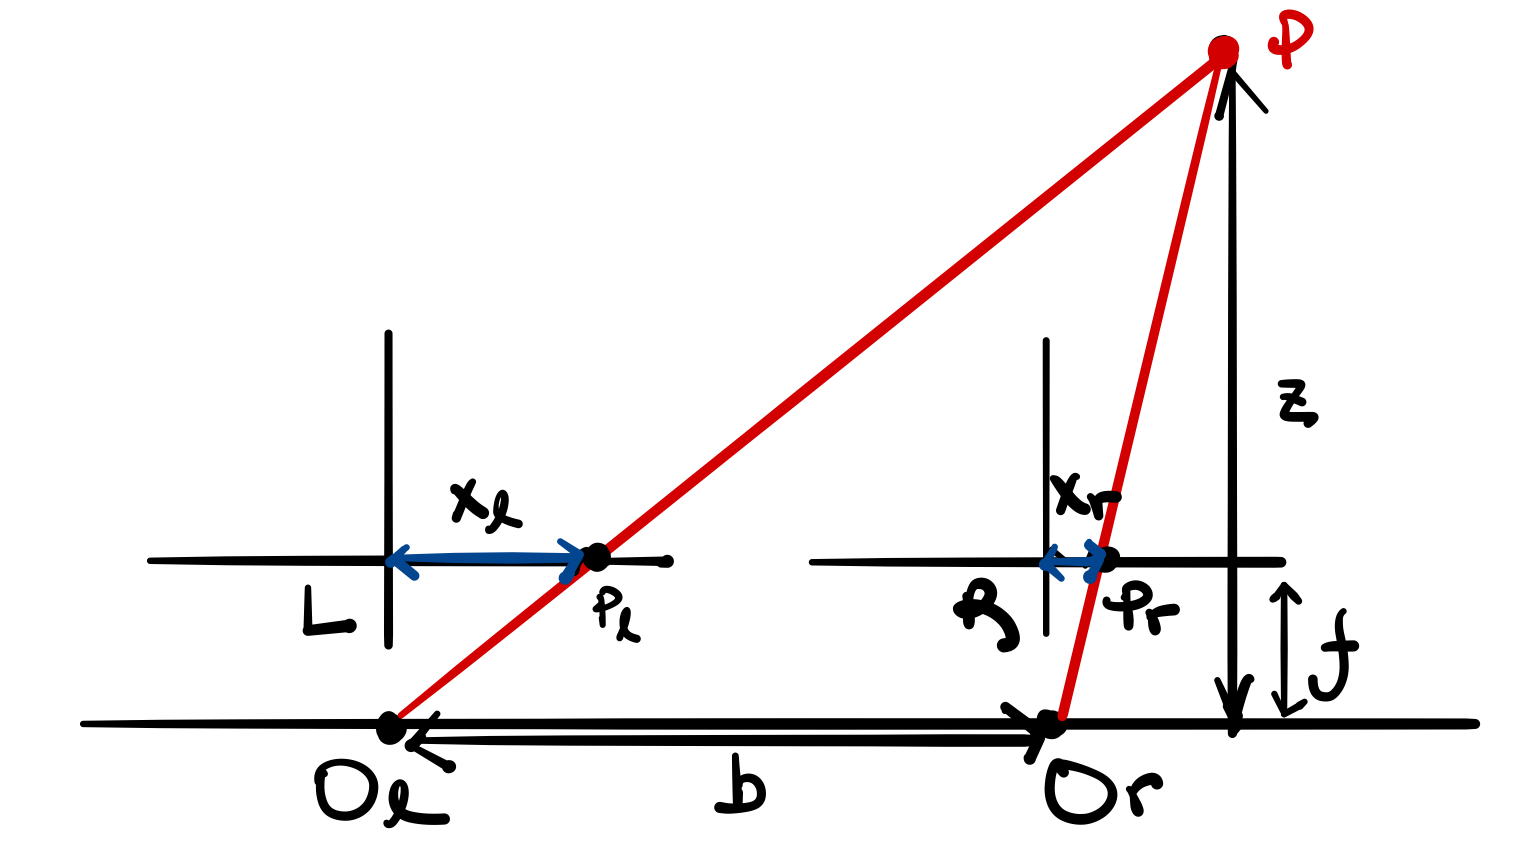
\includegraphics[width=2in]{parallel_camera}
        \caption{parallel-calibrated binocular stereo}
    \end{center}
\end{figure}
\noindent \textit{disparity} is the displacement between points of a conjugate pair $p_l,p_r$ (points in different images of projection of same point in the scene) when the two images are superimposed. In the context of parallel calibrated cameras, disparity is inversely proportional to depth, when baseline $b$ and focal length $f$ are known
\begin{align*}
    \frac{b}{z} = \frac{b + x_l - x_r}{z-f}
    \quad\text{implies}\quad
    z = \frac{bf}{x_l-x_r}
\end{align*}

\subsection{Structured Light Coding}

The goal of structured light coding is to find coding schemes (maps pattern intensity to indices of the projector light planes) that enables robust, reliable algorithms for finding correspondence.


\subsubsection{Horn \& Kiryati} 

This paper generalizes Gray code to n-ary code in order to reduce the number of patterns that needs to be projected, ($L^K$ instead of $2^K$ code words) \cite{hornOptimalStructuredLight1997}. The authors draw inspirations from communication theory, where the projector projects unique temporal codes, received at each image plane through a noisy channel and subsequently decoded. Let there be $K$ patterns and $L$ code words (distinct planes of light), we want to encode the indices of vertical light planes $x\in [L]$ using some encoding scheme $f:[L] \to \R^K$ such that the nearest neighbor decoding $\hat{x}(y) = \argmin_{x\in [L]} ( f(x)-y )^2$ of a normalized noisy observation $y\in\R^K$ minimizes the probability of depth estimation error. Given the forwarding model,
\begin{align*}
    \ry = f(\rx) + \rn
    \quad\quad\text{where}\quad\quad
    \rx 
        &\sim \text{Cat}(1/L)
    \quad
    \rn
        \sim p_{\rn}
\end{align*}
implying $\ry|\rx=x\sim p_{\rn}(y - f(x))$. We want to minimize the probability of depth estimation error, which roughly proportional to difference between true index $x$ of the plane of light and the estimated index $\hat{x}$,
\begin{align*}
    \text{minimize}_{f}\;\; \pb{
        \E_{\rx,\ry} \left[ (x-\hat{x}(y))^2 \right]
        = \sum_{x=1}^L p_{\rx}(x) \int p_{\ry|\rx}(y|x) (x - \hat{x}(y))^2 dy
        \propto \sum_{x=1}^L \int (x-\hat{x}(y))^2 p_{\rn}(y-f(x)) dy
    }
\end{align*}
This optimization problem is hard. The paper suggest the use of space filling curves as the encoding function and established that Gray code is a special limiting case of the space filling curve. Note here we assume there is no \textit{mutual illumination}, i.e. there is no interval reflection and so the projected codes $f(x)$ is proportional to observation $y$. 

\subsubsection{Phase Shifting}

Phase shifting is a particular coding method whereby the projector column coordinates are encoded as the (absolute) phase of a spatial sinusoidal pattern. Note we want to encode column coordinates because we only need to search along the horizontal epipolar lines. Let $N$ be number of columns to be encoded. When the scene is projected with a cosine pattern of period $T$ (measured in number of pixels) and therefore frequency $f=\frac{1}{T}$, an idealized image formation model for any pixel is
\begin{align}
    I 
        = I_0 + A\cos\left( \Phi \right)
        = I_0 + A\cos\left( \phi \right)
    \label{eq:phase_shift_image_formation_one_pixel}
\end{align}
where $I_0$ is the pixel intensity resulting from ambient illumination; $I$ is the pixel intensity measured; $A$ is amplitude (albedo/reflectance) of the signal corresponding to intensity of scene assuming unit intensity for projector patterns; $\Phi = 2\pi f x = 2\pi n + \phi \in [0, 2\pi f N]$ for some number of period $n\in\N$ is the absolute phase, $\phi \in [0,2\pi]$ is the relative phase. When measured w.r.t. number of pixels, $x$ is the corresponding absolute phase and $\tilde{x}$ the corresponding relative phase, satisfying
\begin{align}
    x = Tn + \tilde{x}
    \qquad\text{or}\qquad
    x \equiv \tilde{x} \mod{T}
\end{align}
where $\tilde{x} = \frac{T \phi}{2\pi}$. In (\ref{eq:phase_shift_image_formation_one_pixel}), $I_0,A,\phi$ are unknown and so $\phi$ cannot be determined. To solve for $\phi$, phase shifting method projects $K$ sinusoidal patterns of same frequency, each shifted by $\varphi_k = \frac{2\pi (k-1)}{K}$ for $k=1,\cdots,K$. Thereby obtaining a system of $K$ equations in 3 unknowns. 
\begin{align}
    I_k = I_0 + A\cos\left(\phi + \varphi_k \right)
    \qquad\text{for}\qquad
    k = 1,\cdots,K
    \label{eq:phase_shift_image_formation_one_pixel_shifted}
\end{align}
Although $K=3$ suffices, larger values of $K$ makes determination of relative phase $\phi$ more robust to noise. We determine $\phi$ using least squares
\begin{align}
    \text{minimize}_{\phi}\;\;\pb{
        \epsilon(\phi,I_0,A) := 
            \sum_{k=1}^{K} \pb{
                I_k - \left(
                    I_0 + A\cos\left( \phi + \varphi_k \right)
                \right)
            }^2
    }
    \label{eq:phase_shifting_least_squares}
\end{align}
Similar to appendix in \cite{morenoEmbeddedPhaseShifting2015} and results shown in \cite{pribanicEfficientMultiplePhase2010,morenoEmbeddedPhaseShifting2015}, we can show the following
\begin{align}
    0
        = \frac{\partial \epsilon}{\partial \phi}
        &= 2A \sum_{k=1}^K I_i\sin \left( \phi + \varphi_k \right)
        \propto \cos(\phi) \sum_{k=1}^K I_k \sin(\varphi_k) + \sin(\phi) \sum_{k=1}^{K} I_k \cos(\varphi_k) 
        \nonumber \\
    \phi
        &= \tan^{-1}\pb{
            -
            \frac{
                \sum_{k=1}^K I_k \sin(\varphi_k)
            }{
                \sum_{k=1}^K I_k \cos(\varphi_k)
            }
        }
        \label{eq:phase_shifting_least_squares_solution}
\end{align}
\begin{figure}[h!]
    \begin{center}
        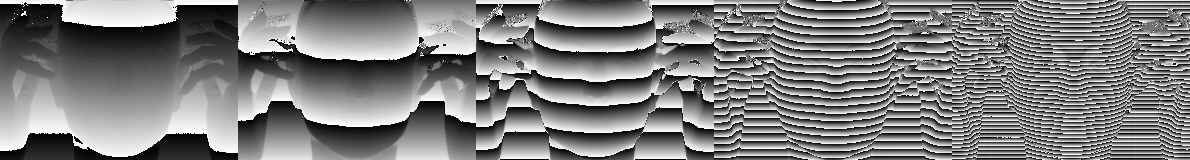
\includegraphics[width=6in]{relphases_1_2_5_17_31}
    \end{center}
    \caption{Relative phase $\phi$ for spatial sinusoids with period 1, 2, 5, 17, 31 solved via (\ref{eq:phase_shifting_least_squares_solution})}
    \label{fig:relative_phase_solution}
\end{figure}

\paragraph{phase unwrapping} aims to recover absolute phase $x$ from relative phase $\tilde{x}$, which is non-trivial unless $T\geq N$. One particular choice of phase unwrapping method relies results in number theory \cite{gushovAutomaticProcessingFringe1991}. The idea is to project patterns whose periods $T_1,\cdots,T_F$ are relative co-prime, each shifted by $K$ times such that relative phase $\tilde{x}_1,\cdots,\tilde{x}_F$ can be solved using (\ref{eq:phase_shifting_least_squares}) or (\ref{eq:phase_shifting_least_squares_u}), from which we can use the Chinese Reminder Theorem to solve a system of congruences
\begin{align}
    x
        &= \tilde{x}_1 \mod{T_1} 
        \nonumber \\
    &\vdots
        \nonumber \\
    x
        &= \tilde{x}_F \mod{T_F} 
    \label{eq:phase_shifting_congruence_system}
\end{align}
Intuitively, projecting $F$ spatial sinusoids with period $T_1,\cdots,T_F$ with different frequency emulates the projection of a low frequency spatial sinusoid with period $T = T_1\times \cdots\times T_F$, shown in Figure (\ref{fig:phase_shifting_emulate_low_freq}). As specified in \cite{guptaMicroPhaseShifting2012} and experimented in Figure (\ref{fig:phase_shifting_not_robust_to_noise}), phase unwrapping is unstable when the relatives phases $\tilde{x}_1,\cdots,\tilde{x}_F$ are noisy. Simple application of medium filtering of the relative phase does not seem to help with phase unwrapping. Wavelet denoising using \texttt{wdenoise} seems to help to a limited extend, as shown in Figure (\ref{fig:phase_shifting_chinese_reminder_lower_freq_noisy_wdenoiser})
\begin{figure}[h!]
    \begin{center}
        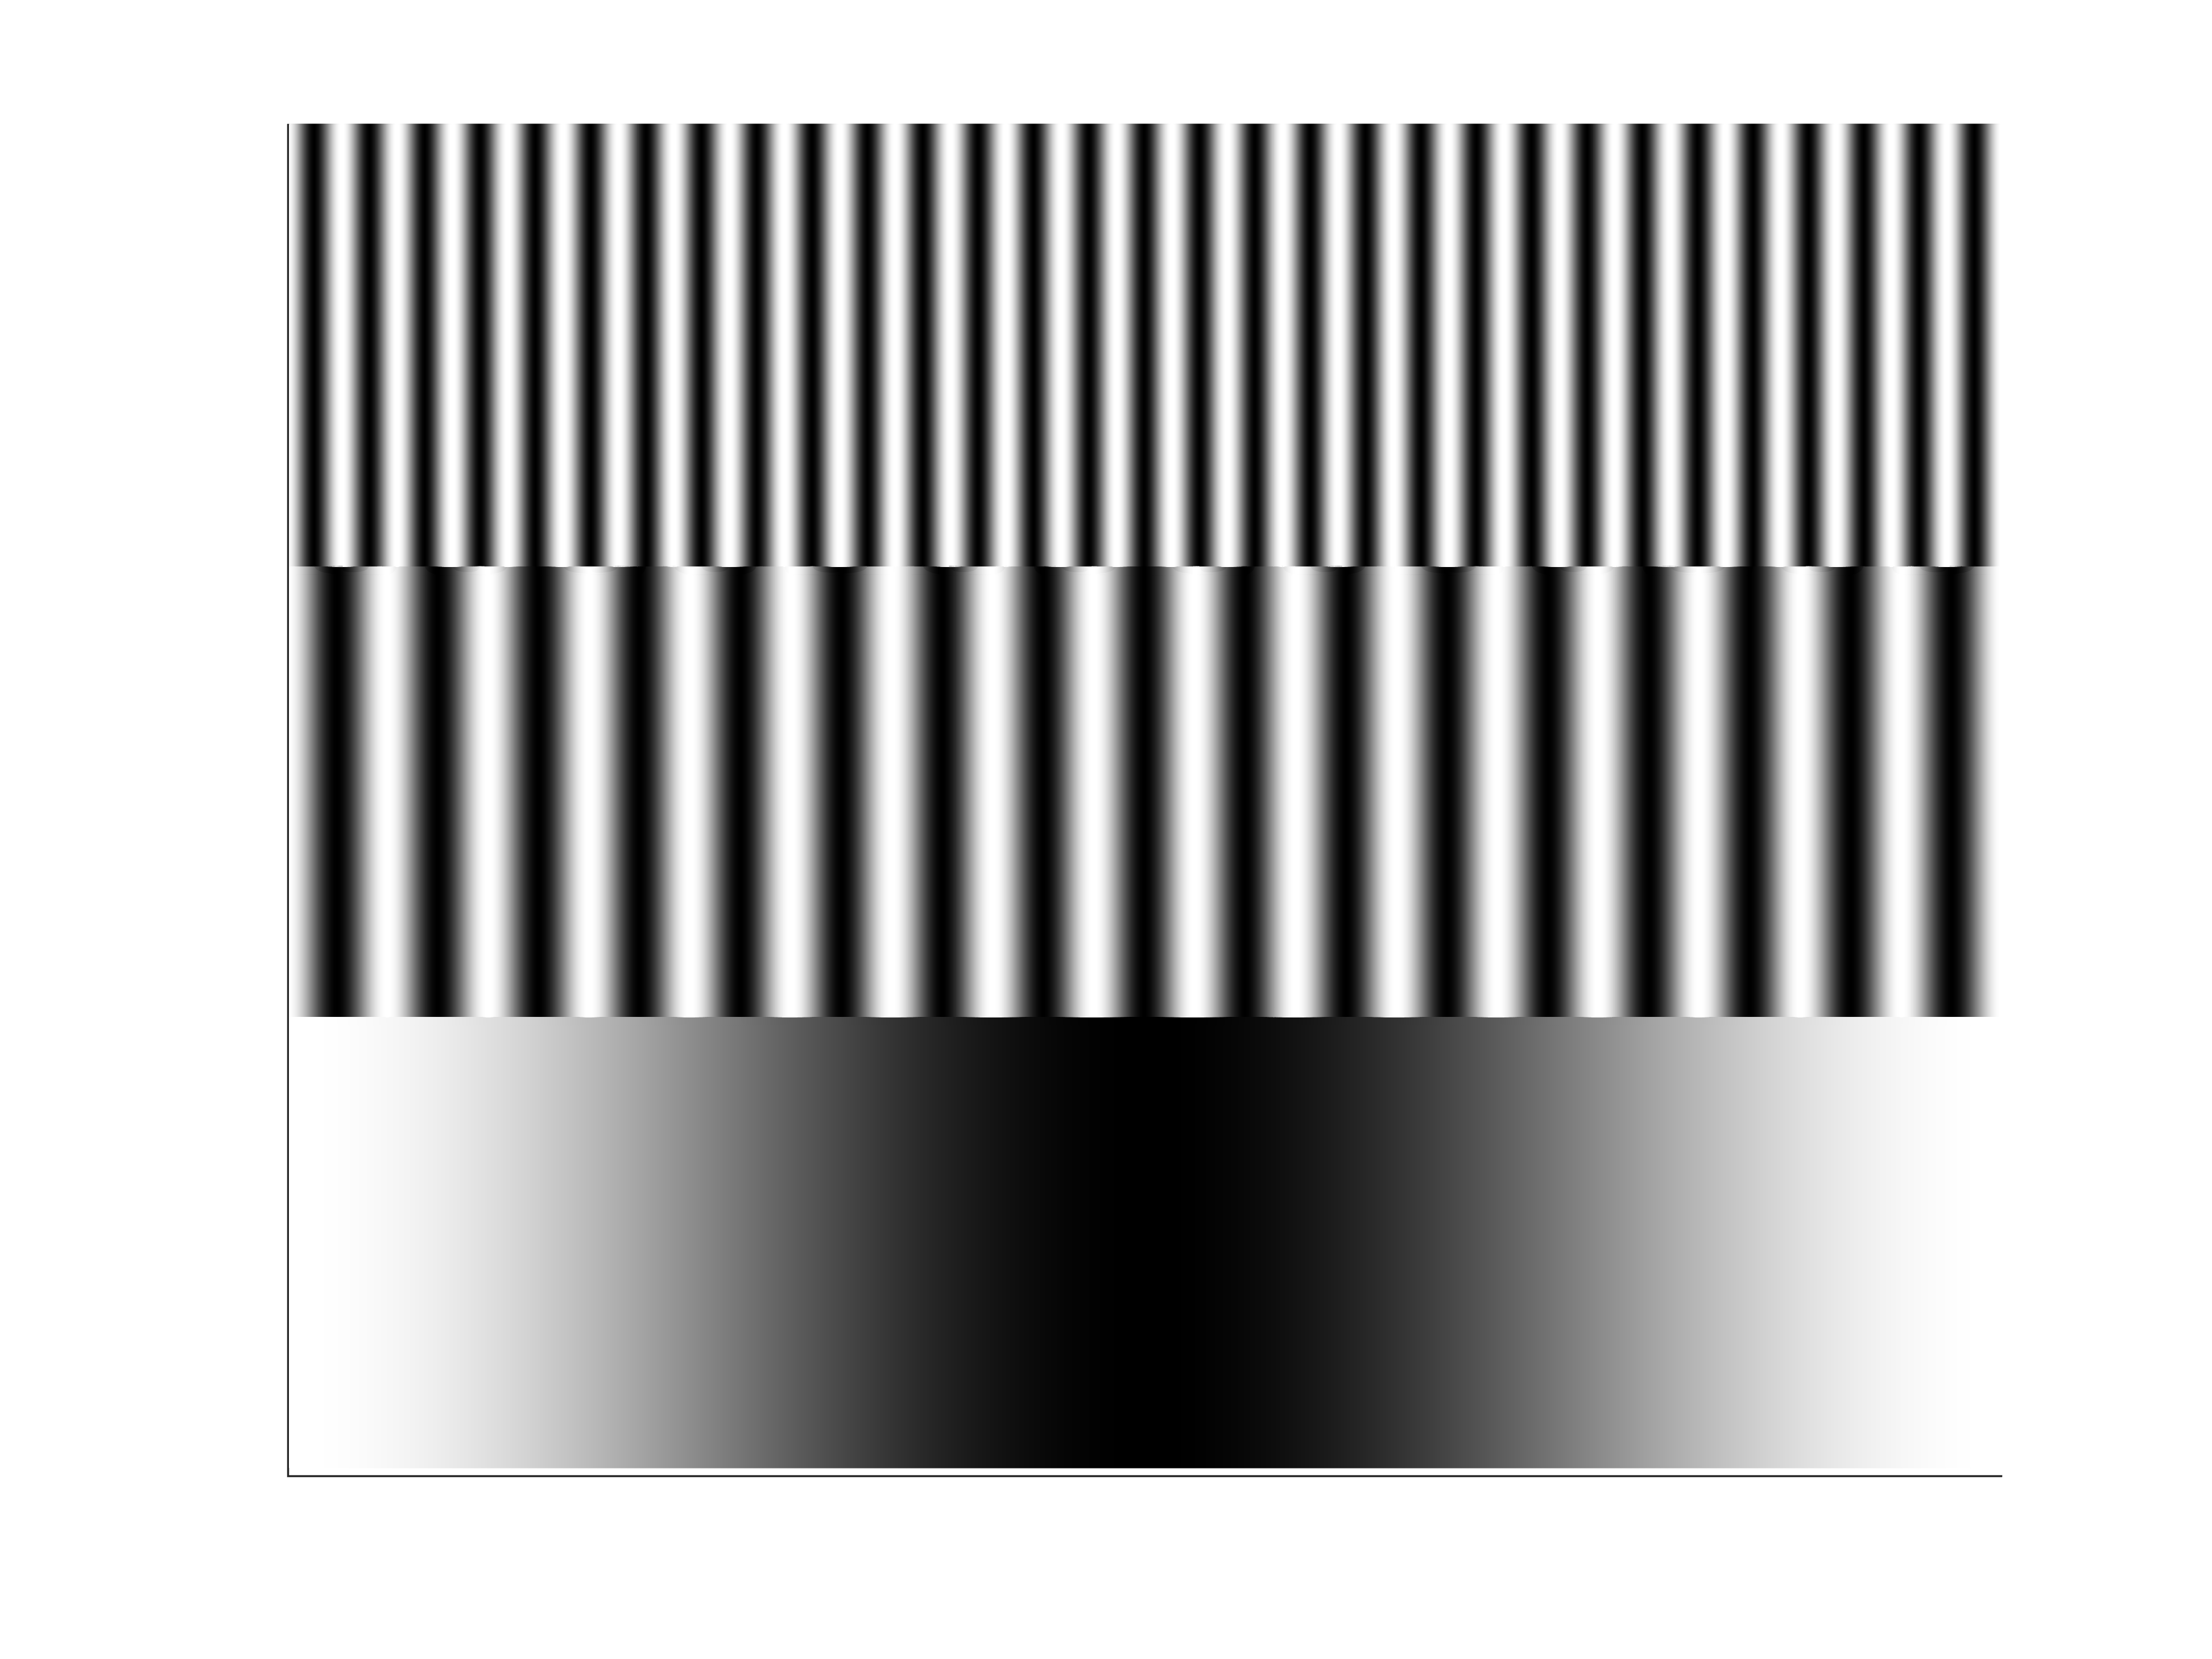
\includegraphics[height=1in,width=5in]{phase_shifting_chinese_reminder_lower_freq}
    \end{center}
    \caption{Two sinusoids with $T_1=17,T_2=31$ emulates a low frequency sinusoid with $T=527$}
    \label{fig:phase_shifting_emulate_low_freq}
\end{figure}
\begin{figure}[h!]
    \begin{center}
        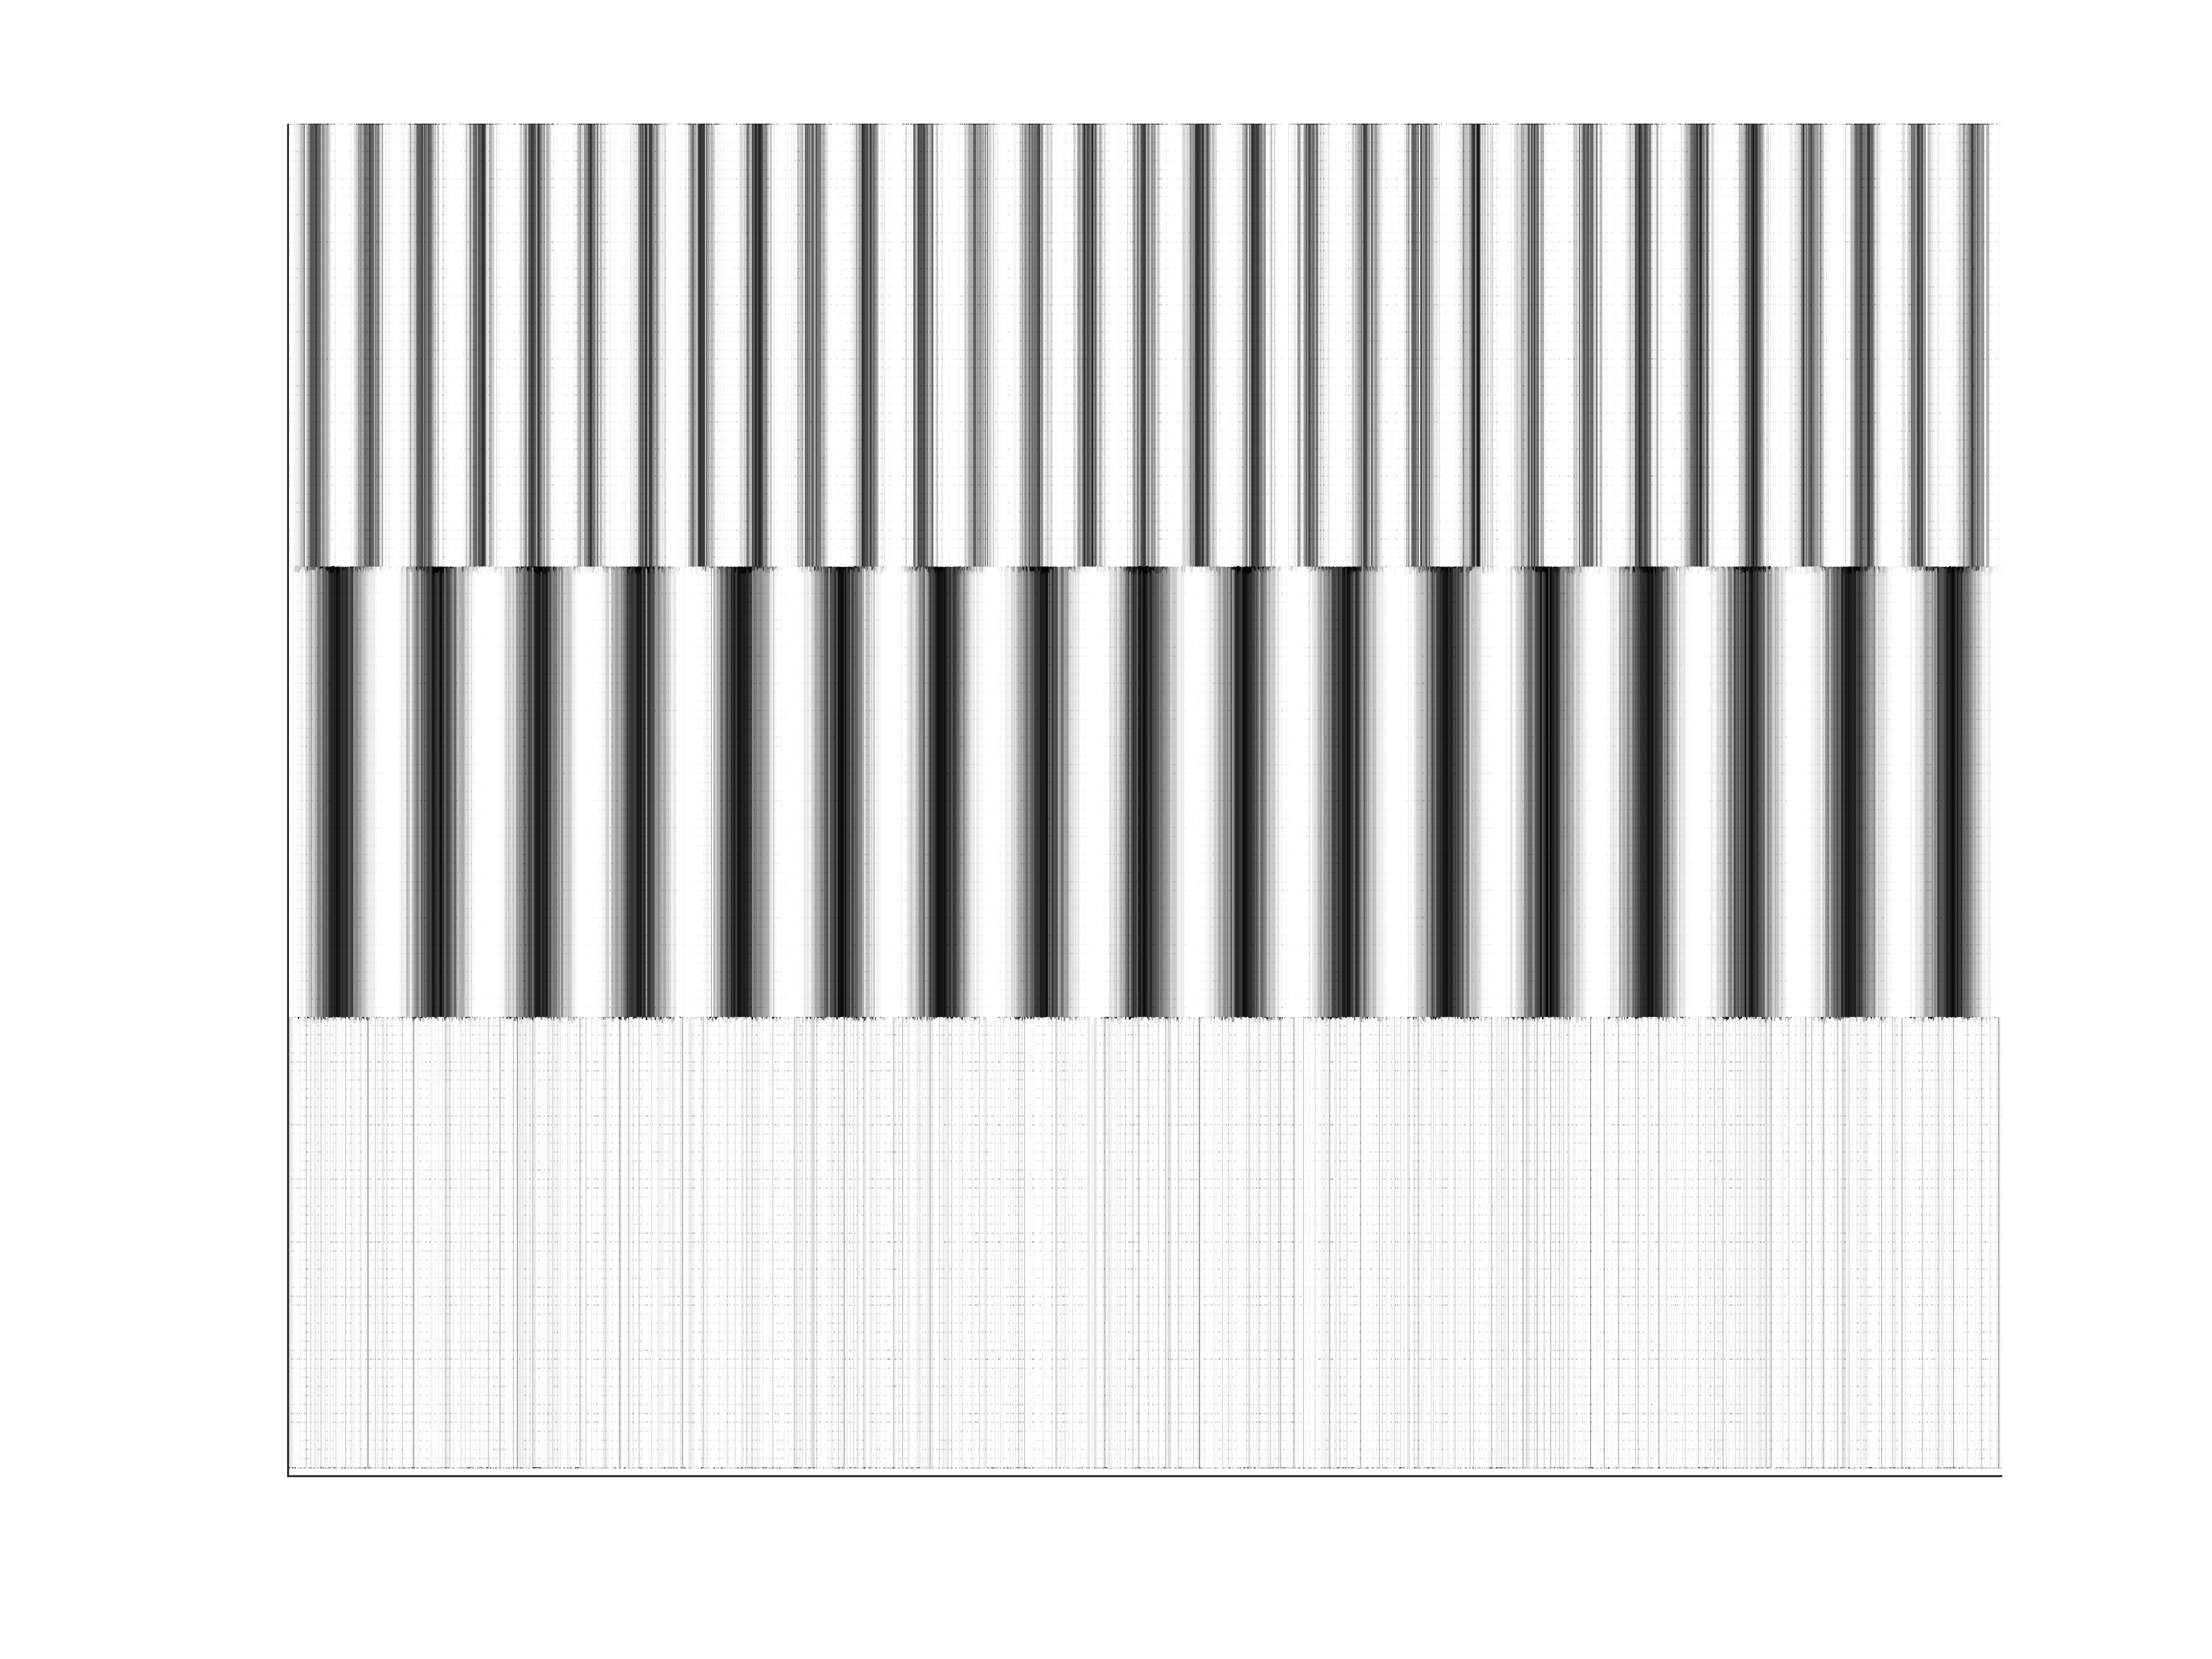
\includegraphics[height=1in,width=5in]{phase_shifting_chinese_reminder_lower_freq_noisy}
    \end{center}
    \caption{When relative phase $\tilde{x}_1,\tilde{x}_2$ are corrupted with i.i.d. additive Gaussian noise $\sN(\boldsymbol{0},0.1 \cdot \textsf{range}(\tilde{x}) \cdot \bI)$, phase unwrapping is unable to recover the absolute phase $x$ robustly.}
    \label{fig:phase_shifting_not_robust_to_noise}
\end{figure}
\begin{figure}[h!]
    \begin{center}
        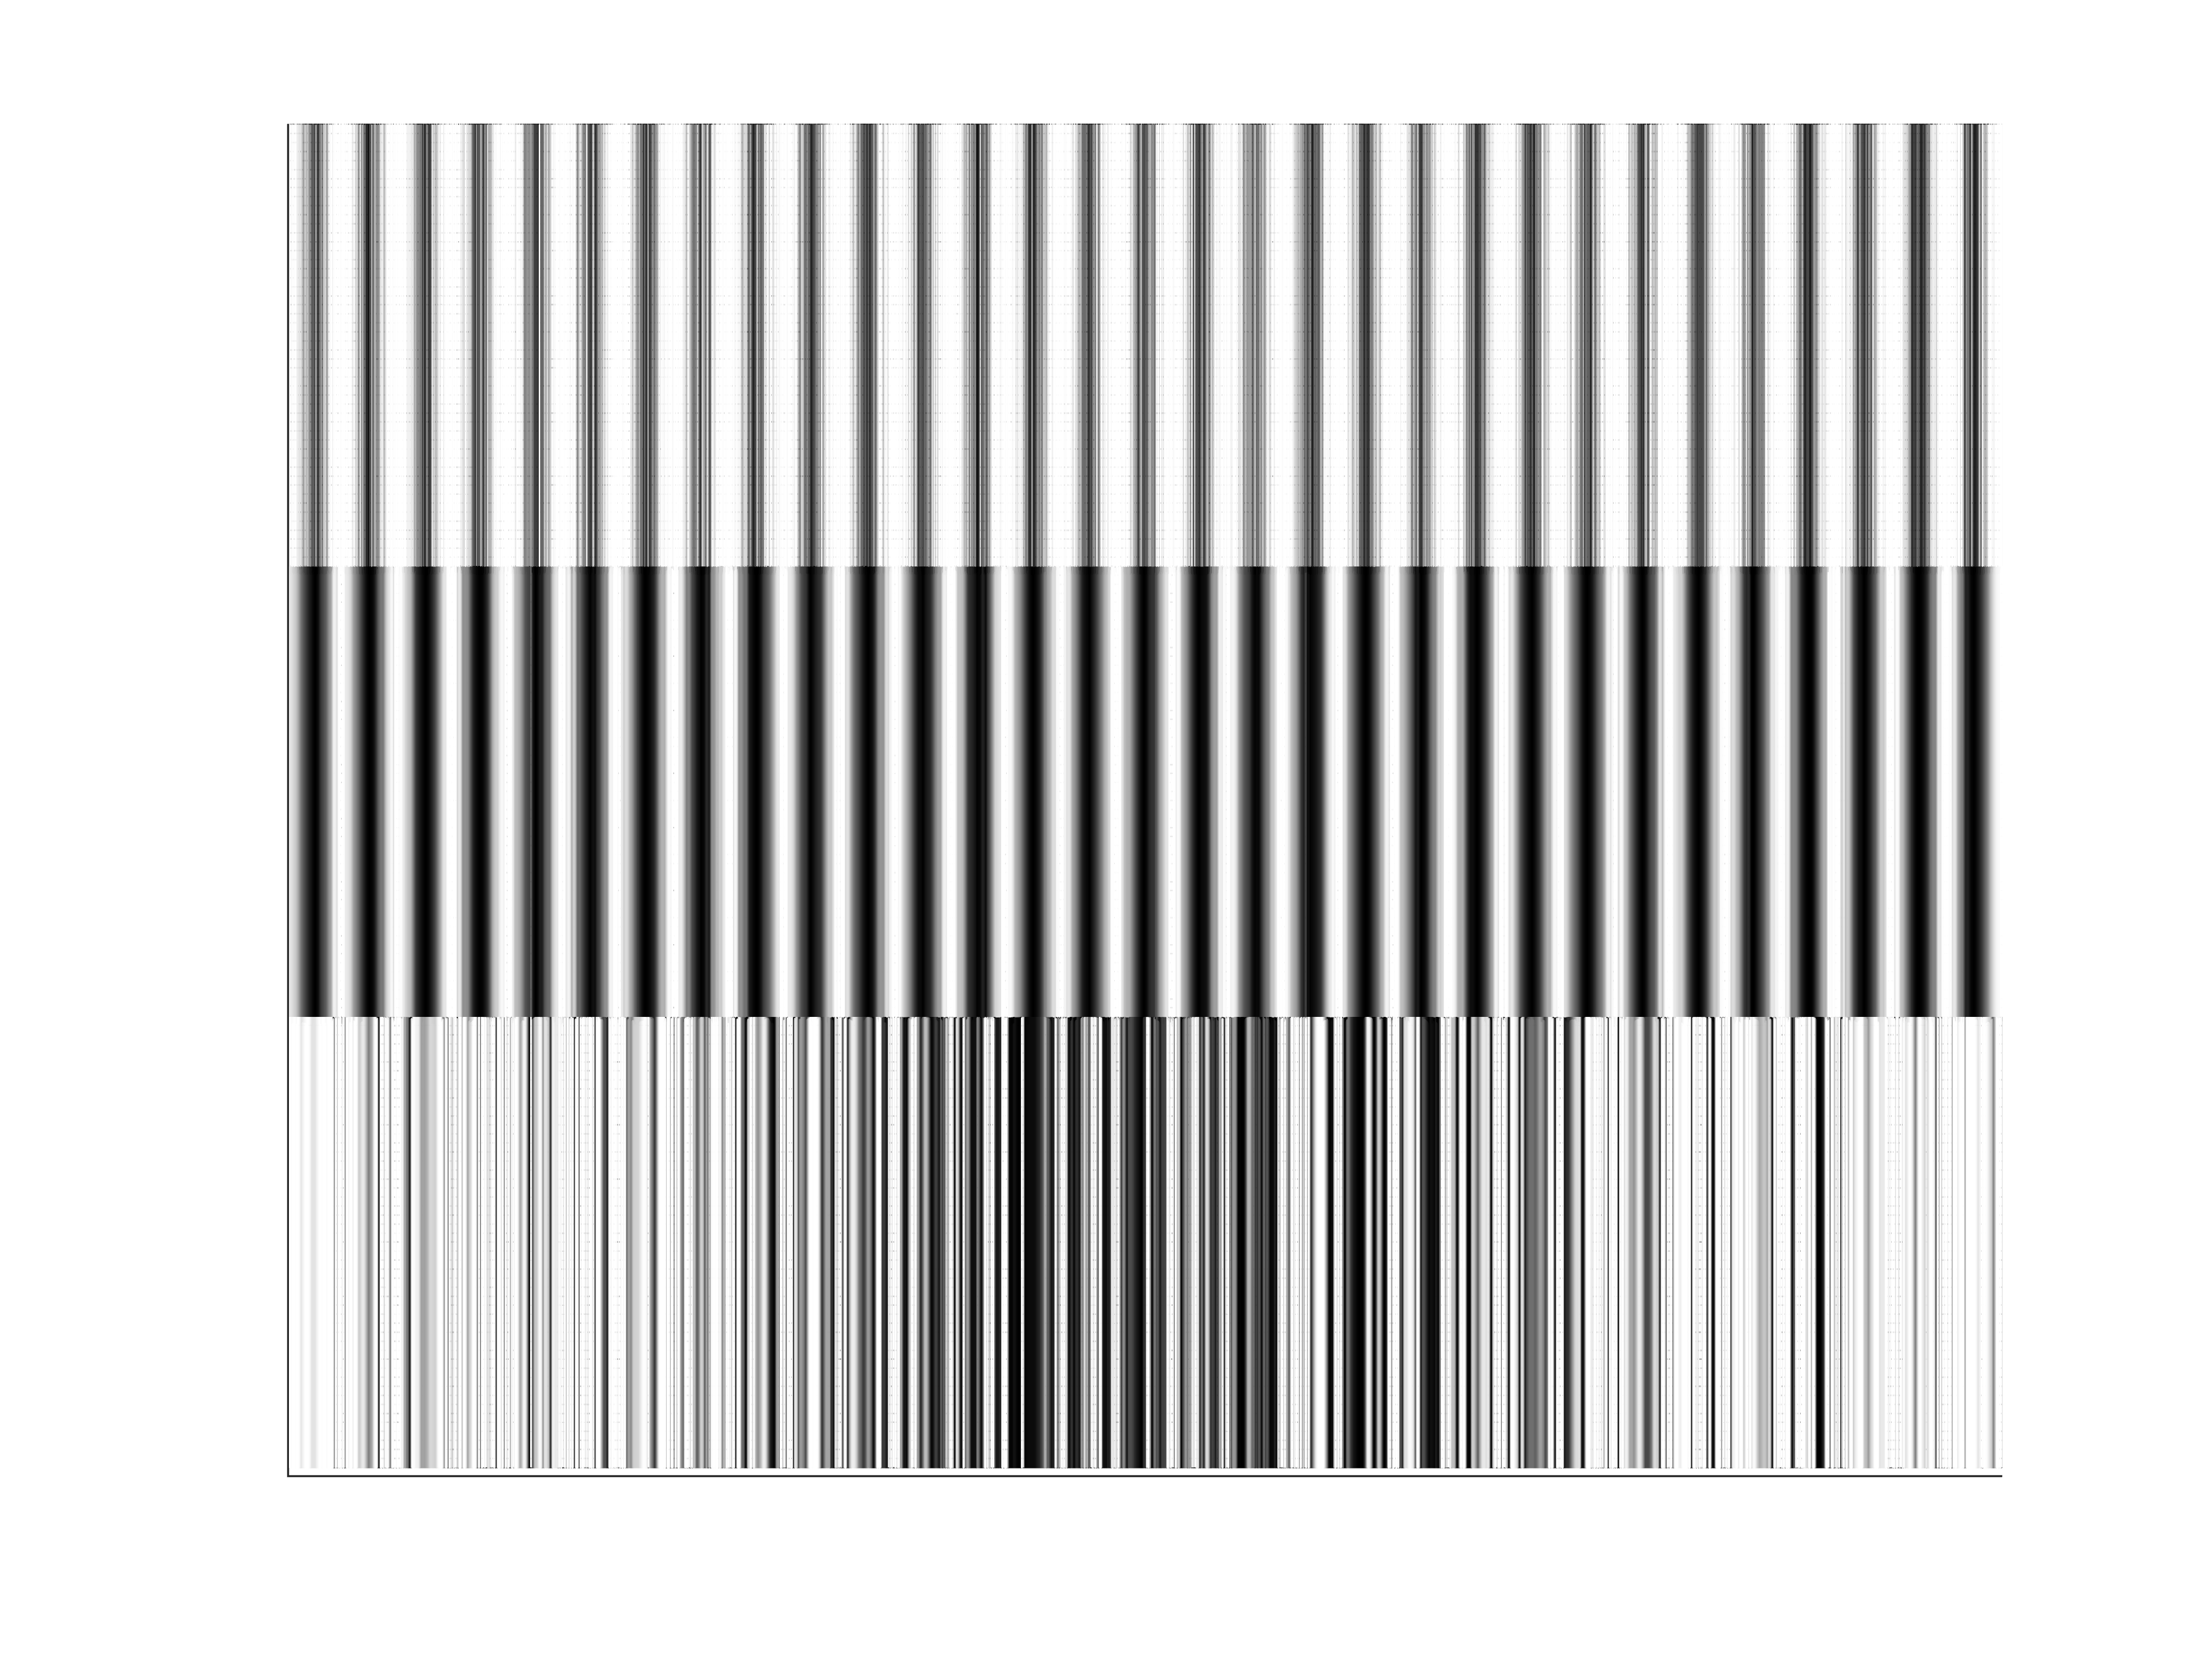
\includegraphics[height=1in,width=5in]{phase_shifting_chinese_reminder_lower_freq_noisy_wdenoiser}
    \end{center}
    \caption{$\tilde{x}_1$ and wavelet denoised $\tilde{x}_1$ ($x_2,\tilde{x}_2$ not shown) helps with phase unwrapping to some extend}
    \label{fig:phase_shifting_chinese_reminder_lower_freq_noisy_wdenoiser}
\end{figure}

\subsubsection{Micro Phase Shifting}
An alternative formulation as mentioned in \cite{guptaMicroPhaseShifting2012}, we can write (\ref{eq:phase_shift_image_formation_one_pixel_shifted}) as a linear system of equations
\begin{align*}
    I_k
        &= I_0 + A\cos(\phi)\cos(\varphi_k) - A\sin(\phi)\sin(\varphi_k)
        = \begin{bmatrix}
            1 & \cos(\varphi_k) & -\sin(\varphi_k)
        \end{bmatrix}
        \begin{bmatrix}
            I_0 \\ A\cos(\phi) \\ A\sin(\phi)
        \end{bmatrix} \\
    \underbrace{
        \begin{bmatrix}
            I_1 \\ \vdots \\ I_K
        \end{bmatrix}
    }_{\bI}
        &= 
        \underbrace{
            \begin{bmatrix}
                1 & \cos(\varphi_1) & -\sin(\varphi_1) \\
                \vdots & \vdots & \vdots \\
                1 & \cos(\varphi_K) & -\sin(\varphi_K) \\
            \end{bmatrix}
        }_{\bM}
        \underbrace{
            \begin{bmatrix}
                I_0 \\ A\cos(\phi) \\ A\sin(\phi)
            \end{bmatrix}
        }_{\bu}
\end{align*}
and solve for $\bu$ using least squares,
\begin{align}
    \text{minimize}_{\bu}\;\;
        \norm{\bI-\bM\bu}_2^2
    \label{eq:phase_shifting_least_squares_u}
\end{align}
The relative phase is then given by
\begin{align*}
    \phi 
        = \cos^{-1}\left( \frac{\bu_2}{A} \right)
    \qquad\text{where}\qquad
    A
        = \sqrt{\bu_2^2 + \bu_3^2}
    \quad\text{and}\quad
    \bu
        = M^{\dagger} \bI
\end{align*}
Note the optimization problem formulated in (\ref{eq:phase_shifting_least_squares},\ref{eq:phase_shifting_least_squares_u}) are not equivalent. 

\subsubsection{ZNCC Decoding}

Let $L$ be number of vertical light planes to be encoded, $f:[L]\to\R^K$ is some encoding scheme that encodes index $x$ to a code $f(x)$, $y$ is per pixel measurement. Similar to nearest neighbor decoder used in \cite{hornOptimalStructuredLight1997}
\begin{align}
    \hat{x}(y)
        = \argmin_{x\in [L]} \left( f(x) - y \right)^2
    \label{eq:nearest_neighbor_decoder}
\end{align}
\cite{mirdehghanOptimalStructuredLight2018} defines a decoding function that is optimal in a sense in small noise regimen,
\begin{align}
    \hat{x}(y)
        = \argmax_{x\in[L]} \textsf{ZNCC}\left( y, f(x) \right)
    \label{eq:zncc_decoder}
\end{align}
Note the quality of decoding depends heavily on the noise level. Additionally, number of shifts is crucial for good reconstruction of absolute phase, see Figure~\ref{fig:disparity_vs_random_shifts}
\begin{figure}[h!]
    \begin{center}
        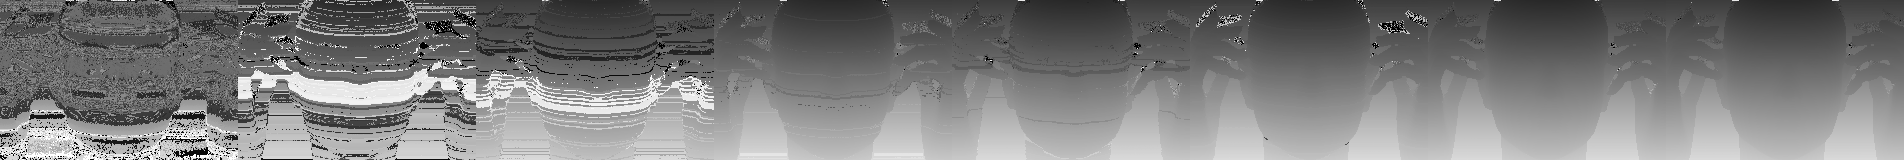
\includegraphics[width=7in]{disparity_vs_shifts_3_5_7_10_12_15_50_149_}
    \end{center}
    \caption{Here we have spatial sinusoids with period 1,2,5,17,31, each shifted 30 times projected onto a static scene. Resulting in $5\cdot 30=150$ measurement, each stacked from 250 noisy images. We see ZNCC decoding taking 3,5,7,10,12,15,50,150 randomly chosen measurements respectively yield progressively better disparity reconstruction}
    \label{fig:disparity_vs_random_shifts}
\end{figure}
\begin{figure}[h!]
    \begin{center}
        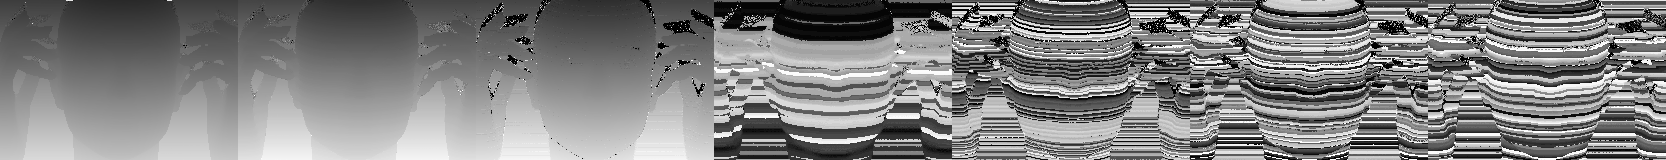
\includegraphics[width=7in]{zncc_decoding_phase}
        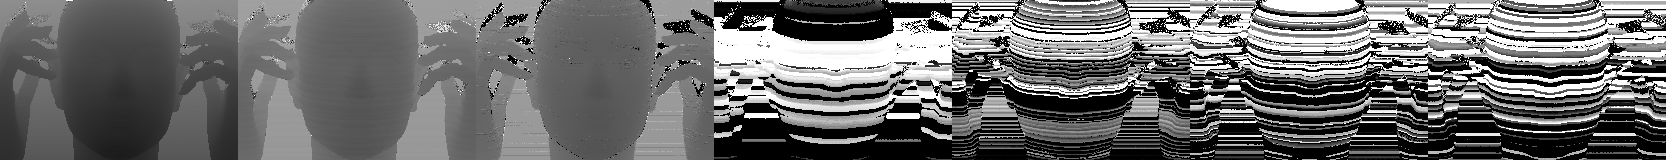
\includegraphics[width=7in]{zncc_decoding_disparity}
    \end{center}
    \caption{ZNCC decoded phase and disparity for (from left to right) ground truth shown in Figure~\ref{fig:disparity_vs_random_shifts}, Hamiltonian, MPS, Optimized-MDE, Optimized-Top0, Optimized-Top1, Optimized-Top2. Apart from ground truth, reconstruction takes intensity of scene under 7 projector patterns, each stacked from 250 noisy measurements}
    \label{fig:zncc_decoding_phase_disparity}
\end{figure}

\subsubsection{Geometric Perspective \& Hamiltonian Code} 
 
When trying to find optimal encoding scheme that minimizes bayesian decoding/correspondence error, a surrogate objective is the length of the coding curve. \cite{guptaGeometricPerspectiveStructured2018} argues that an optimal coding scheme should have a coding curve that is long, non-intersecting, and distance preserving (points far along the curve should also be far in euclidean distance). Sinusoidal codes has intersection with itself, i.e. multiple column indices are coded to the same location in measurement space implying there is $2\pi$ phase ambiguity when trying to compute its inverse decoding function. The distance preserving property is especially important in noisy regime, where non-distance preserving coding scheme would potentially yield large error as the decoding function maps (w.r.t. Euclidean distance) noisy measurement to indices far away from true value. For example, A La Carte code is not distance preserving as shown in Figure~\ref{fig:coding_curve_la_carte}. 
\begin{figure}[h!] 
    \begin{center}
        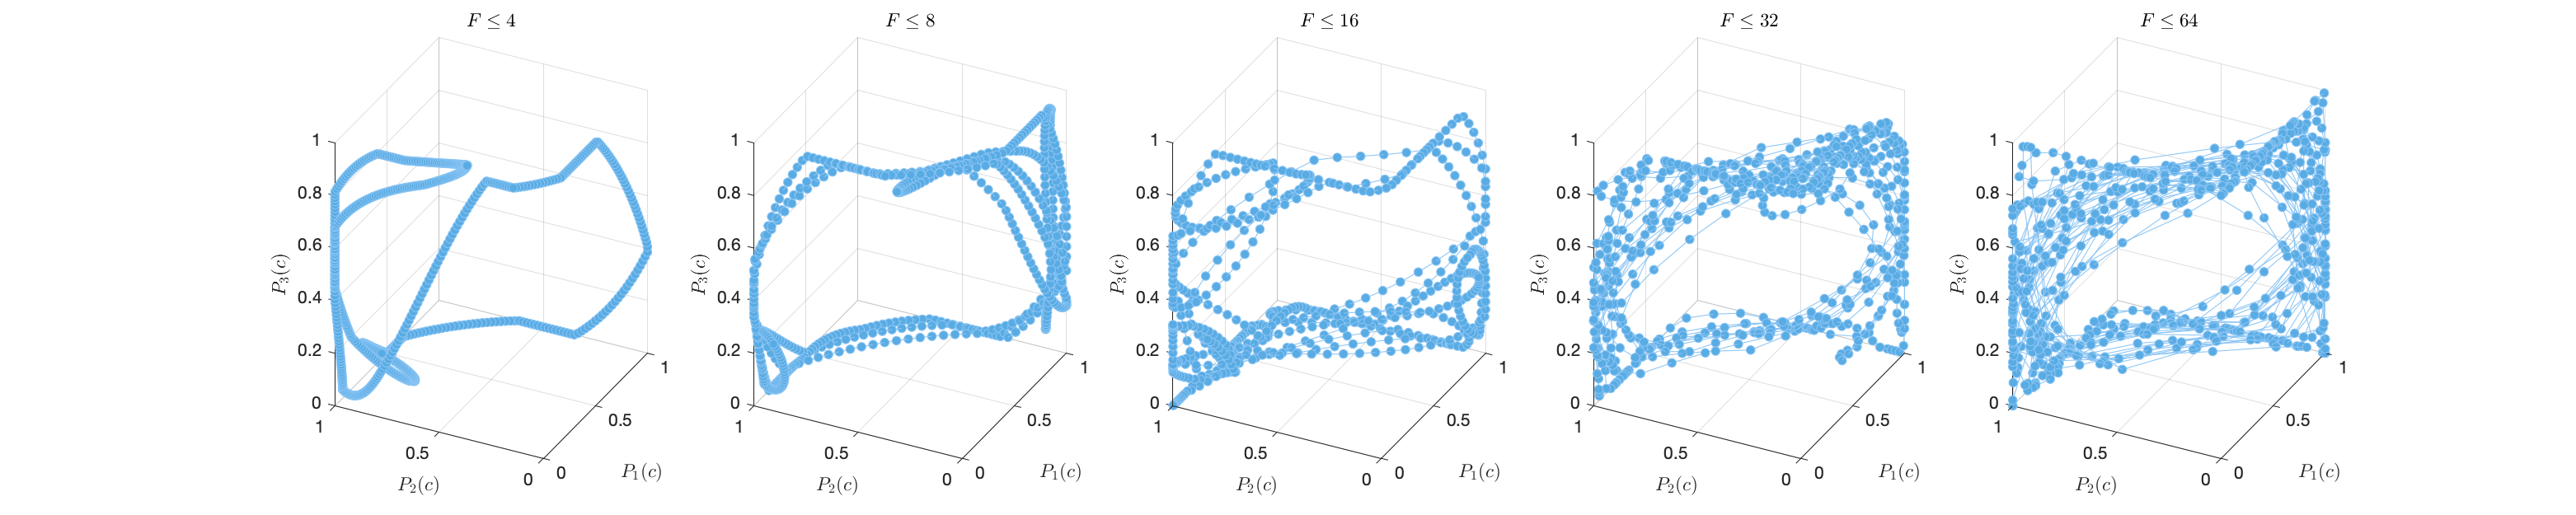
\includegraphics[height=3cm]{coding_curve_la_carte}
        \caption{A La Carte codes for $3$ patterns with varying max spatial frequency \cite{mirdehghanOptimalStructuredLight2018} is not distance preserving, i.e. points far along the curve are close in measurement space in the Euclidean sense. So we'd expect it to have sub-optimal performance when measurements are noisy}
        \label{fig:coding_curve_la_carte}
    \end{center}
\end{figure}
\begin{figure}[h!]
    \begin{center}
        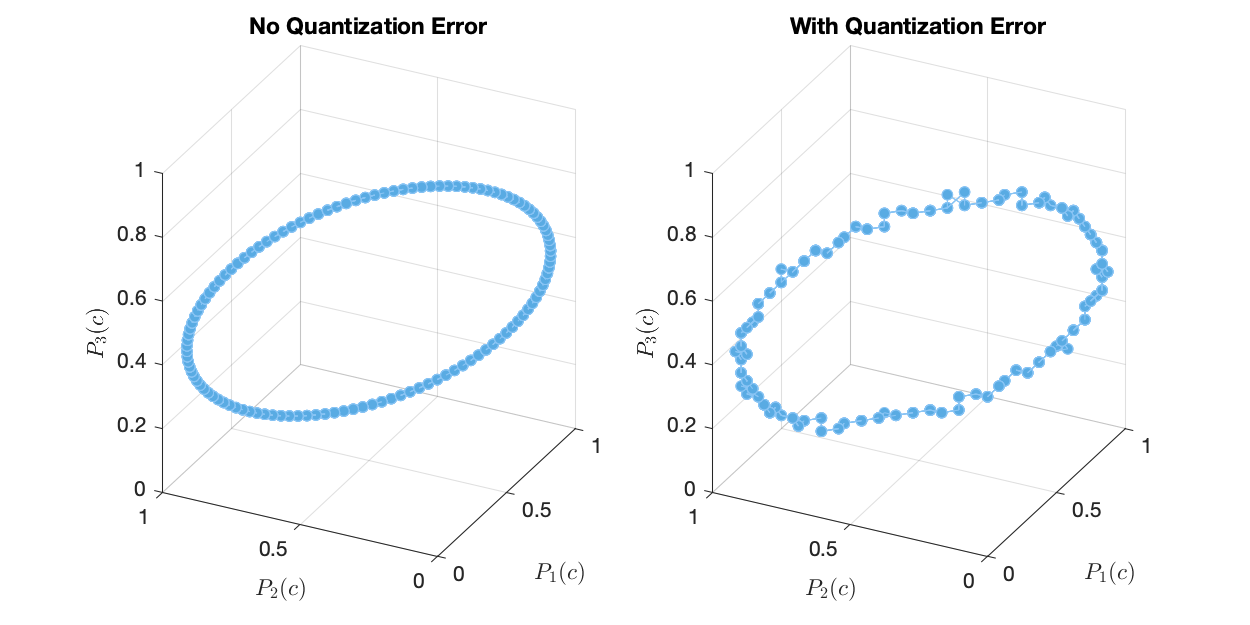
\includegraphics[height=5cm]{coding_curve_quantization_effect}
        \caption{Projector quantization error translates to jitters in the coding curve for sinusoidal patterns}
        \label{fig:coding_curve_quantization_effect}
    \end{center}
\end{figure}
\begin{figure}[h!]
    \begin{center}
        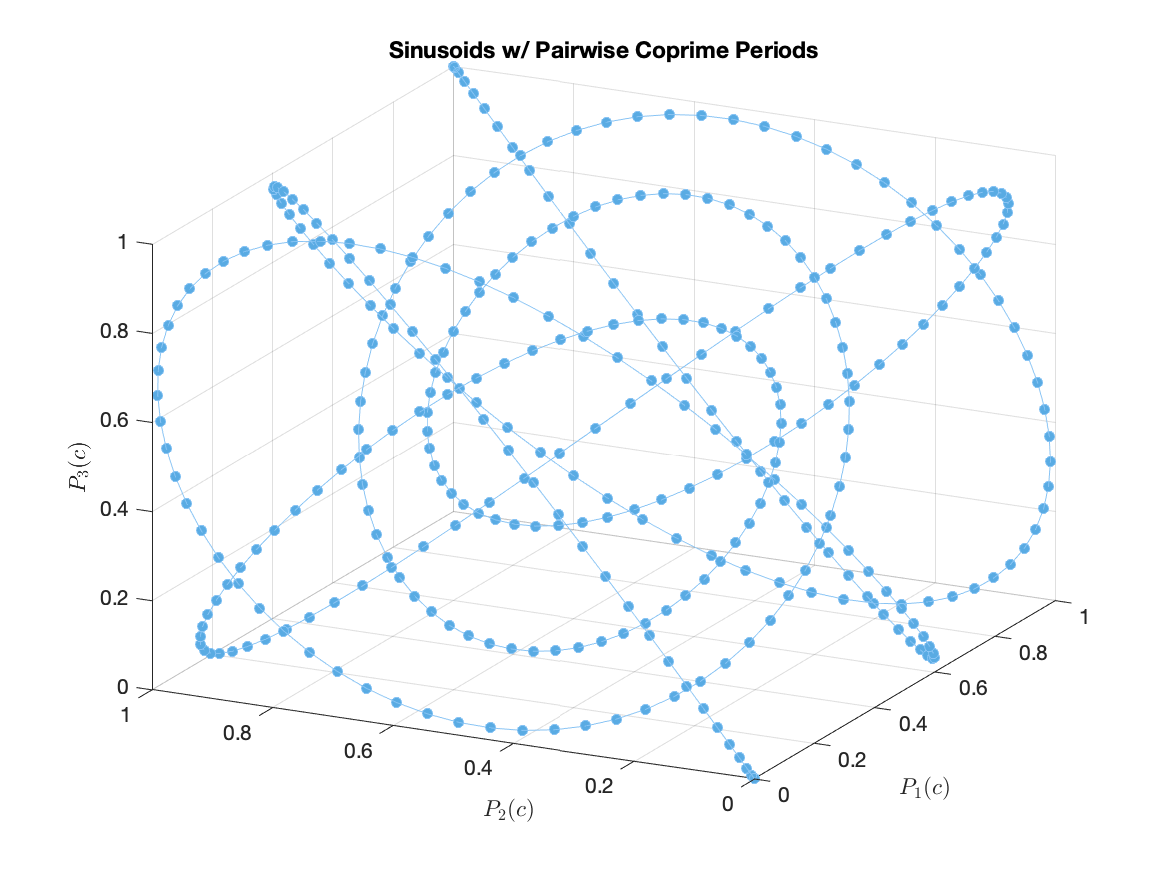
\includegraphics[height=5cm]{coding_curve_sinusoids_pairwise_coprime}
        \caption{Sinusoids with pairwise co-prime periods (5, 11, 13) is non-intersecting and therefore emits unique decoder using the Chinese Reminder Theorem. However, certain points along the curve does not satisfy the distance preserving property, implying the code is not optimal when measurements are noisy. For sinusoidal codes, non-intersection and distance preserving is a conflicting objective so it seems.}
        \label{fig:coding_curve_sinusoids_pairwise_coprime}
    \end{center}
\end{figure}


\subsection{Alternating Direction Method of Multipliers}

\subsubsection{Formulation}

Consider the following equality constrained convex optimization problem 
\begin{align}
    \text{minimize}\;
        &f(x) + g(z) \\
    \text{subject to}\;
        &Ax+Bz=c
    \label{eq:admm_objective}
\end{align}
assuming $f,g$ are both convex. The augmented lagrangian $L_{\rho}$ makes the objective better behaved,
\begin{align}
    L_{\rho}(x,z,y)
        &= f(x) + g(z) + y^T\left(Ax + Bz - c\right) + \frac{\rho}{2} \norm{Ax+Bz-c}_2^2
\end{align}
where $y$ is the dual variable, and $\rho>0$ is the penalty parameter. The method of multipliers is simply doing gradient ascent (using $\rho$ as stepsize) on the dual objective computed from the augmented lagrangian
\begin{align}
    (x^{k+1},z^{k+1})
        &= \argmin_{x,z} L_{\rho}(x,z,y^{k}) 
        \label{eq:method_of_multiplier_minimization} \\
    y^{k+1}
        &= y^k + \rho \nabla L_{\rho}(x^{k+1},z^{k+1},y)
        = y^k + \rho \left( Ax^{k+1} + Bz^{k+1} - c \right)
        \label{eq:method_of_multiplier_dual_update}
\end{align}
When regular lagrangian is used and when objective is separable, the minimization step (\ref{eq:method_of_multiplier_minimization}) is also separable with respect to the primal variables $x,z$. The addition of Euclidean norm on the residual of primal equlity constraints makes the optimization coupled. ADMM is method of multiplier where a single Gauss-Seidel pass over the primal variable is used instead of jointly optimizing for $x,z$.
\begin{align}
    x^{k+1}
        &= \argmin_{x} L_{\rho}(x,z^k,y^k) 
        \nonumber \\
    z^{k+1}
        &= \argmin_{z} L_{\rho}(x^{k+1},z,y^k) 
        \nonumber \\
    y^{k+1}
        &= y^k + \rho \left( Ax^{k+1} + Bz^{k+1} - c \right)
        \label{eq:admm_iterates_dual_update}
\end{align}
We can gather the residual term $r=Ax+Bz-c$ and completing the squares and get
\begin{align}
    L_{\rho}(x,z,y)
        = f(x) + g(z) + \frac{\rho}{2} \norm{Ax + Bz - c + u}_2^2
    \label{eq:admm_scaled_augmented_lagrangian}
\end{align}
where $u=\frac{1}{\rho}y$ is scaled dual variable. The scaled form ADMM is then
\begin{align}
    x^{k+1}
        &= \argmin_x \pb{
            f(x) + \frac{\rho}{2} \norm{Ax+Bz^k-c+u^k}_2^2 
        } 
        \nonumber \\
    z^{k+1}
        &= \argmin_z \pb{
            g(z) + \frac{\rho}{2} \norm{Ax^{k+1}+Bz-c+u^k}_2^2
        } 
        \nonumber \\
    u^{k+1}
        &= u^k + Ax^{k+1} + Bz^{k+1} - c
    \label{eq:admm_scaled_form}
\end{align}

\subsubsection{LASSO Problem}

The lasso problem is 
\begin{align}
    \minimize\;
        & \frac{1}{2} \norm{Ax-b}_2^2 + \lambda \norm{x}_1
    \label{eq:lasso_unconstrained_problem}
\end{align}
We can apply variable splitting and obtain an equivalent constrained optimization problem
\begin{align}
    \minimize
        & \frac{1}{2} \norm{Ax-b}_2^2 + \lambda \norm{x}_1 \\
    \subjectto
        & x - z = 0
    \label{eq:lasso_unconstrained_problem}
\end{align}
Specialize (\ref{eq:admm_scaled_form}) to lasso to obtain iterates of the form
\begin{align}
    x^{k+1}
        &= \left( A^TA + \rho I \right)^{-1} \left( A^Tb + \rho(z^{k} - u^k) \right) \\
    z^{k+1}
        &= \sS_{\lambda/\rho} \left( x^{k+1} + u^k \right) \\
    u^{k+1}
        &= u^k + x^{k+1} - z^{k+1}
\end{align}
which essentially performs lasso ($x$ update) repeatedly.



\subsubsection{Affine Constrained Convex Optimization Problem}
\begin{equation}
    \begin{aligned}
        \underset{\bx_1,\cdots,\bx_N}{\minimize}
            &\pb{f(\bx) = \sum_{i=1}^N f_i(\bx_i)} \\
        \subjectto
            & (\bx_1,\cdots,\bx_N) \in \sC \\
    \end{aligned}
    \label{eq:constrained_cvx}
\end{equation}
where $\bx_i\in\R^{n_i}$, $f_i: \R^{n} \to (-\infty,\infty)$ are closed proper convex functions for $i=1,\cdots,N$. Here we assume $\sC = \{ \bx \in\R^{n_1\times \cdots\times n_N} \;\mid\; A \bx = \bb \}$ is an affine set. (\ref{eq:constrained_cvx}) has an equivalent form,
\begin{equation}
    \begin{aligned}
        \underset{\bx,\bz}{\minimize}  & f(\bx) + \delta_{\sC}(\bz) \\
        \subjectto & \bx - \bz = 0 \\
    \end{aligned}
    \label{eq:constrained_cvx_indicator_set}
\end{equation}
which can be solved using ADMM iterates of the form,
\begin{align*}
    \bx_i^{k+1} 
        &= \argmin_{\bx_i} \left( f_i(\bx_i) + \frac{\rho}{2} \norm{\bx_i - (\bz_i^k - \bu_i^k)}_2^2 \right) 
        = \prox_{(1/\rho)f_i}(\bz_i^k - \bu_i^k) \\
    \bz^{k+1}
        &= \argmin_{\bz} \left( \delta_{\sC}(\bz) + \frac{\rho}{2} \norm{ \bz - (\bx^{k+1} + \bu^k) }_2^2 \right)
        = \prox_{(1/\rho)\delta_{\sC}}(\bx^{k+1} + \bu^k) \\
    \bu^{k+1} 
        &= \bu^k + \bx^{k+1} - \bz^{k+1}
\end{align*}
where $\prox_{\lambda f}: \R^n \to \R^n$ is the proximal operator of $\lambda f$, $\lambda >0$, 
\[
    \prox_{\lambda f}(\bv) = \argmin_{\bx} \left( f(\bx) + \frac{1}{2\lambda} \norm{\bx-\bv}_2^2 \right)    
\]

\subsubsection{Some Common Proximal Operator}

Evaluating the proximal operator involves solving a convex optimization problem. We will show how we can compute the proximal operators relevant to our methods. (See section 6 of \cite{parikhProximalAlgorithms2014}) 

\paragraph{Projection Onto Convex Set} 
The proximal operator of an indicator function onto a convex set $\sC$ is simply the projection onto $\sC$. 
\[
    \prox_{(1/\rho)\delta_{\sC}}(\bx^{k+1} + \bu^k) =  \textstyle\prod_{\sC}(\bx^{k+1}+\bu^k)
\]
When $\sC$ is affine, there is an analytic expression for the projection
\begin{align*}
    \textstyle\prod_{\sC}(\bv) 
        &= \bv - A^{\dagger}(A\bv-\bb)  \\
        &= \bv - A^T(A^TA)^{-1}(A\bv-\bb) \tag{if $A\in\R^{m\times n}$ has $m<n$ and full rank}
\end{align*}

\paragraph{Quadratic Function}

Let $f$ be $\ell$-2 norm of an affine function, assuming $A\in\R^{p\times n}$
\[
    f(x) 
        = \frac{1}{2} \norm{A\bx-\by}_2^2 
        = \frac{1}{2}\bx^TA^TA\bx - \by^TA\bx + \frac{1}{2}\by^T\by
\]
Then proximal operator of $(1/\rho)f$ has a closed form expression
\[
    \prox_{(1/\rho)f}(\bv) 
        = (\rho I + A^TA)^{-1} (\rho \bv + A^T \by)
\]
which can be solved efficiently with conjugate gradient, as $(\rho I + A^TA) \succ 0$. If $\rho$ is fixed throughout, we can use Cholesky factorization to factor $(\rho I + A^TA)$ in $\sO(n^3)$. Any subsequent computation of the inverse with back-solve would only cost $\sO(n^2)$. When $p<<n$, we can exploit this by using the matrix inversion lemma, 
\[
    (\rho I + A^TA)^{-1} 
        = \frac{1}{\rho} I - \frac{1}{\rho} A^T \left( \rho I + AA^T \right)^{-1} A
\]
The dominant cost is computing $(AA^T)^{-1} \in \R^{p\times p}$. Each $x$ update now costs $\sO(np^2)$. If use Cholesky factorization to factor $(\rho I + AA^T)$ once, subsequent iteration can be carried out in $\sO(np)$ flops, which is essentially costs for matrix-vector multiply.

\paragraph{$\ell$-1 Norm} 
Let $f(\bx) = \norm{\bx}_1$, then the proximal operator of $\lambda f$ is
\[
    \prox_{\lambda f}(\bv) 
        = \sS_{\lambda}(\bv)
\]
where $\sS$ is element-wise soft shrinkage operator
\[
    (\sS_{\lambda}(\bv))_i
        = (1-\lambda/|\bv_i|)_{+}\bv_i
    \quad\quad
    \bx_{+} = \max(\bx,0)
\]

\paragraph{RED Explicit Regularizer}

Let $f(\bx) = (1/2)\bx^T(\bx-\sD(\bx))$ for some denoiser $\sD$, the explicit regularizer in RED.\cite{romanoLittleEngineThat2016}. We use one fixed point iteration evaluate the approximate proximal operator for $\lambda f$. Specifically, we want to evaluate 
\[
    \prox_{(\lambda/\rho)f} (\bv)
        = \argmin_{\bx} \frac{\lambda}{2}\bx^T(\bx-\sD(\bx)) + \frac{\rho}{2} \norm{\bx-\bv}_2^2
\]
Setting the gradient to zero, we arrive at the fixed point iteration
\[
    \bx^{(k)} \leftarrow \frac{1}{\rho+\lambda}(
        \lambda \sD(\bx^{(k-1)}) + \rho \bv
    )
\]
If we only iterate once, then 
\[
    \prox_{(\lambda/\rho)f} (\bv)
        = \frac{1}{\rho+\lambda}( \lambda \sD(\bx^{(0)}) + \rho \bv )
\]
for some initialization value $\bx^{(0)}$



\subsection{Linear Inverse Problem}

Numerous inverse problem in image processing are modeled using the following relationship
\[
    y = Ax + \epsilon   
\]
wherer $y\in\R^m$ is noisy measurement, $x\in\R^n$ are unknown image, $A \in \R^{m\times n}$ captures the forward relationship, $\epsilon\in\R^m$ is noise. The goal is to estimate $x$ from noisy $y$ by making assumptions about the noise distributioon $\epsilon$ and exploiting structure in the latent variable $x$.


\subsubsection{MAP inference under Gaussian Noise}

A typical approach to solve the linear inverse problem relies on computing max a posterior (MAP) estimator while assuming somer prior distirbution $p_{\rx}$. In particular given observation $y$, we want to estimate $\hat{x}$ where
\begin{align}
    \hat{x}
        = \argmax_{x} p_{\rx|\ry}(x|y)
    \label{eq:inverse_problem_map_problem}
\end{align}
Assuming isotropic Gaussian noise $\epsilon \sim \sN(0,\sigma^2 I)$, the conditional likelihood depends on the noise distribution, $\ry\mid \rx=x \sim \sN(Ax, \sigma^2 I)$. The log likelihood is then
\begin{align*}
    \log p_{\ry|\rx}(y|x)
        = -\frac{m}{2} \log (2\pi) - \frac{1}{2\sigma^2} \norm{Ax - y}_2^2 
\end{align*}
Then the problem (\ref{eq:inverse_problem_map_problem}) reduces to
\begin{align}
    \hat{x}
        = \argmax_{x} \pb{
            \log p_{\ry|\rx}(y|x) + \log p_{\rx}(x) 
        }
        = \argmin_{x} \pb{
            \frac{1}{2\sigma^2} \norm{Ax-y}_2^2 - \log p_{\rx}(x)
        }
\end{align}







\newpage

\subsection{Image Priors} 






The choice of regularization has been an important research topic in image processing. Handcrafted priors have been successful in a number of different image recovery tasks. For example, we can choose to enforce task-specific priors: (1) the sparsity of $\bx$ with $\ell$-1 norm in image deblurring \cite{beckFastIterativeShrinkageThresholding2009} (2) total variation in image denoising \cite{buadesNonlocalImageMovie2008} (3) cross-channel correlation in color image demosaicing \cite{malvarHighqualityLinearInterpolation2004} (4) dark channel prior in image dehazing \cite{fattalSingleImageDehazing2008}, etc. More exhotically, randomly initialized neural network can inject inductive bias to the optimization and act as image priors. \cite{ulyanovDeepImagePrior2017}

$ $\\
In addition to hand-crafted priors, there has been interest in algorithm induced priors. Alternating direction method of multipliers (ADMM) is a common convex optimization method for inverse problem where the objective function is separable with respect to the \textit{data term} and the \textit{regularizer}. Each primal update involves an evaluation of a proximal operator, which can be interpreted as performing denoising on some iterate. \cite{venkatakrishnanPlugandPlayPriorsModel2013,heideFlexISPFlexibleCamera2014,chanAlgorithmInducedPriorImage2016} proposed plug-and-play priors where the choice of regularization is implicitly specified by the denoiser used. \cite{romanoLittleEngineThat2016} proposed an explicit laplacian-based expression for the regularizer and generalizes the method to a number of different iterative optimization algorithms.

$ $\\
The convergence of plug-and-play ADMM is studied by a number of papers. \cite{chanPlugandPlayADMMImage2016} showed fixed point convergence of plug-and-play ADMM. \cite{romanoLittleEngineThat2016} showed convergence of the algorithm under some mild conditions of the denoiser, which are satisfied by some state of the art denoisers like \textit{Block-matching and 3D filtering
 (BM3D)} \cite{dabovImageDenoisingSparse2007} and \textit{Trainable Nonlienar Reaction Diffusion (TNRD)} \cite{chenTrainableNonlinearReaction2017}. Most recently, \cite{ryuPlugandPlayMethodsProvably2019} established convergence given that the denoising network satisfy certain Lipschitz condition.

$ $\\ 
Some proposed to learn proximal operator from data. \cite{meinhardtLearningProximalOperators2017} used a CNN denoiser \cite{zhangGaussianDenoiserResidual2017}. Instead of substituting the proximal operator with a denoiser, \cite{changOneNetworkSolve2017} learns a projection mapping to the space of natural images by training a single neural network and showed impressive results on a number of different linear inverse problems.



\end{document}
